% Metódy inžinierskej práce

\documentclass[10pt,oneside,slovak,a4paper]{article}

\usepackage[slovak]{babel}
%\usepackage[T1]{fontenc}
\usepackage[IL2]{fontenc} % lepšia sadzba písmena Ľ než v T1
\usepackage[utf8]{inputenc}
\usepackage{graphicx}
\usepackage{url} % príkaz \url na formátovanie URL
\usepackage{hyperref} % odkazy v texte budú aktívne (pri niektorých triedach dokumentov spôsobuje posun textu)
\usepackage{pdfpages}
\usepackage{cite}
%\usepackage{times}

\pagestyle{headings}

\title{Hry pre zdravie ako súčasť každodenného života\thanks{Semestrálny projekt v predmete Metódy inžinierskej práce, ak. rok 2022/23, vedenie: Ing.Igor Stupavský}} % meno a priezvisko vyučujúceho na cvičeniach

\author{Kristián Červenka\\[2pt]
	{\small Slovenská technická univerzita v Bratislave}\\
	{\small Fakulta informatiky a informačných technológií}\\
	{\small \texttt{xcervenkak@stuba.sk}}
	}

\date{\small 19. september 2022} % upravte



\begin{document}

\maketitle

\begin{abstract}
V tomto článku som sa preto rozhodol zamerať na vnášanie gamifikácie do oblasti zdravotníctva a využitie hier pre zdravie a ich vplyv v oblasti bežného života ľudí.
Objasním, čo sú to vlastne hry pre zdravie a ako vedia byť prospešné pre vývoj dieťaťa.
Ďalej by som sa chcel zamerať na zlepšenie životného štýlu používateľov hier pre to určených.Objasním hry pre zdravie na akom princípe fungujú a čo je zároveň ich cieľom.
Objasním princíp fungovania hier pre zdravie, ich cieľ a implementáciu v každodennom živote.
Spracujem tému ako sú hry jednou zo schopností ako prinútiť ľudí byť flexibilný , respektíve viacej sa hýbať v dnešnom technologickom svete a zároveň sa proaktívne vysporiadať s rýchlo meniacim svetom technológií. 
Hry sú jednou z možností ako zmeniť ľudské správanie na prijateľnejšie pre spoločnosť preto sa zameriam aj na hry pre psychické zdravie.
\end{abstract}



\section{Úvod}
Videohry ponúkajú inovatívne, vzrušujúce a vysoko efektívne metódy na zvyšovanie vedomostí a ovplyvňovanie zdravotných výsledkov. 
V 21.storočí rastie potreba chrániť zdravie ľudí prostredníctvom variácie dostupných zdrojov.
Jednou z možností ako zlepšiť zdravie ľudí pohybujúcich sa po tomto svete je zasadenie gamifikácie do prostredia zdravotníctva. 
Pre spracovanie témy som sa rozhodol z dôvodu nárastu dopytu hier hre zdravie.Videohry majú schopnosť zaujať používateľov inou cestou ako iné média.
V oblasti zdravotníctva sa videohry objavili v rôznych oblastiach. 
Za posledných dvadsať rokov sa používajú v odbornom výcviku, terapii, starostlivosti o seba, podpore zdravia i v komunikácii o zdraví.


\section{Motivácia} 
\subsection{Hry pre zdravie}
Videohry vo všeobecnosti majú schopnosť zaujať hráčov iným spôsobom ako ponúkajú dnešné novodobé média.Hry sa stávajú zaujímavou oblasťou rôznych výskumov a pokusov predvádzaných vedcami. Zo štúdie asociovanej Entertainment Software Association \cite{PLP-Framework} vyplýva , že približne 29\% hráčov sú v rozmedzí 18 a menej rokov. 
V súčastnosti využívame sofistikované technológie na podporu zdravia spôsobom , ktorý bol nepredstaviteľný pre minulé generácie.Množstvo hier pre zdravie je postavených na platformách dávno známych hráčom , ako sú napríklad osobné počítače alebo webové stránky.Hry podnecujú ich používateľov k opakovanému hraniu a preukazujú postupné  pozitívne zmeny správania potrebné na dosiahnutie individuálnych zdravotných zmien.
\subsection{Moderné pokroky v oblasti hier pre zdravie}
Vývoj a testovanie prebieha v širokom spektre chorôb , na prevenciu a liečbu zdravotných problémov.Bolo vykonaných množstvo výskumov zameraných na zdravotný stav človeka, akými sú napríklad cystická fibróza,liečba bolesti , Parkinsonova choroba , obezita a rôzne variácie vírusových ochorení.Tento výskum zahŕňal mimo iných i psychické  choroby a rehabilitácie, akými sú napríklad depresia, posttraumatická stresová porucha , úzkosť , popáleniny , mŕtvica,traumatické poškodenia mozgu a mnohé iné.Príkladom sú sociálne problémy , s ktorými sa ľudstvo stretáva takmer každý deň, násilie , šikanovanie , rasové predsudky\cite{bworld}.
\label{nejaka}
\section{Modifikácie hier pre zdravie v oblastiach bežného života}

\subsection{Hry ako forma edukácie prospešná pre vývoj dieťaťa}
Hry sú formou rekreácie, ktorá sa vo všeobecnosti považuje za prospešnú pre rozvoj dieťaťa. Vo väčšine prípadov majú hry pravidlá , ciele, možnosti voľby, výzvy a body , ktoré od mala nabádajú dieťa ku základným pravidlám spoločnosti. Príkladom sú seriózne hry , ktoré sú navrhnuté tak , aby mimo zábavy vniesli do života i iný účel.Tím vedcov zaoberajúci sa hrami o zdraví kategorizoval tieto hry do najmänej štyroch kategórií.Individálnou kategóriou hier pre zdravie sú hry určené na školenia zdravotníkov poskytujúcich zdravotnú starostlivosť. Herný dizajn ponúka mimo iného i prvky herného dizajnu , ktoré sú atraktívne pre rôzne vekové skupiny. Medzi základné prvky herného dizajnu patria napríklad interaktivita a spätná väzba. Pomocou nej majú možnosť hráči ihneď po inicializovaní akcie dostať okamžité informácie a ich dôsledok. Mimo iných majú hráči možnosť vyberať si identitu , pomocou ktorej získajú schopnosť stať sa hernou postavou a vytvoriť si vzťah a prepojenie s inými postavami v hre.
\begin{enumerate}
    \item{Implementácia zdravotných hier v oblasti edukácie.}
    \item{Zmeny správania zapríčinené hrami pre zdravie}
    \item{Fyzická aktivita obsiahnutá v obsahu hier pre zdravie}
    \item{Hry pre zdravie ovplyvňujúce zdravotné prekurzory}
\end{enumerate}
%\section{Modifikácie hier pre zdravie v oblastiach bežného života}
\paragraph{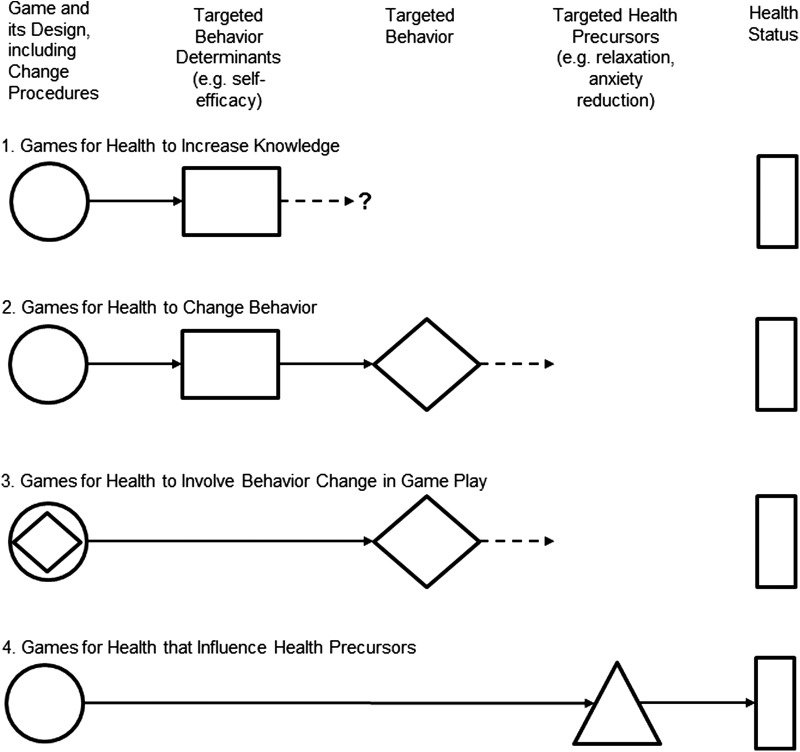
\includegraphics[scale=2]{tps_1.jpeg}}
\caption{1.obr Rozdelenie hier pre zdravie}

\subsection{1.Implementácia zdravotných hier v oblasti edukácie}
Mnohé zahraničné štúdie preukázali prepojenie zážitkových,herných, a vedomostných aspektov ako jednu z najlepších foriem učenia vôbec pre zapojenie študentov do akademických , zdravotných a spoločenských tématických oblastí.Zo štúdií vyplynulo , že hry ktoré ponúkajú možnosť učenia prostredníctvom ich hrania sú účinnejšie v metaanylýze 39 štúdií a umožňujú študentom lepšiu edukáciu ako tradičná výučba z hľadiska zapamätania si informácii z pohľadu študentov.Učitelia uvádzali , že vážne hry boli z hľadiska zapamätania informácií obzvlášť motivujúce pre študentov so slabými až mierne priemernými výsledkami,avšak toto samotné zvýšenie vedomostí nemusí viesť ku zlepšeniu zdravotného stavu.Napriek tomu , že herné výučbové technológie nie sú príliš rozširené, nedávny výskum ukázal , že až 55\% učiteľov využíva hry na skvalitnenie vzdelania svojich žiakov aspoň raz týždenne.Avšak medzi prvoradé prekážky využívania hier na edukáciu patrí najmä nedostatok času, vysoké náklady a nedostatok technologických prostriedkov v triedach.Dopomáhajú tomu i normy a požiadavky , ktoré vývojárom hier sťažujú DevOps hier určených na výučbu.

\begin{table}[!ht]
    \centering
    \scalebox{0.7}{
    \begin{tabular}{|l|l|l|l|}
    \hline
        Dôvody nevyužívania hier v oblasti edukácie & ~ & Implementácia hier pre zdravie v oblasti edukácie a ich efektivita & ~ \\ \hline
        Názov problému & Početnosť & Názov dôvodu & Efektivita \\ \hline
        Nedostatok času & 45\% & Motivácia do učenia & 61\% \\ \hline
        Peniaze & 44\% & Zlepšenie reflexov & 57\% \\ \hline
        Nedostatok technických zdrojov & 35\% & Spríjemnenie procesu vzdelávania & 53\% \\ \hline
        Nevyhovujúce hry pre výučbu & 34\% & Súťaživosť & 49\% \\ \hline
        Dôraz na štandardizáciu výsledkov testov & 29\% & Naučenie pravidiel & 45\% \\ \hline
        Nevedomosť hľadania kvalitných hier & 27\% & Kooperácia medzi študentami & 68\% \\ \hline
        Nestotožnenosť učiteľov s technológiami & 23\% & Edukácia vyhovujúca každému typu študenta & 32\% \\ \hline
        Nedostatok podpory od štátu & 14\% & Naučenie orientácie v spoločnosti & 48\% \\ \hline
        Žiadne dôvody & 7\% & Myslenie v hraničných situáciách & 25\% \\ \hline
        Iné dôvody & 4\% & Zlepšenie jazykovej zložky a všeobecného prehľadu & 11\% \\ \hline
    \end{tabular}

    }
    \caption{Dôvody nevyužívanie hier v oblasti edukácie a ich efektivita}
\end{table}

\subsection{2.Zmeny správania zapríčinené hrami pre zdravie}
Prvý vykonaný prieskum rôznych hier pre zdravie preukázal , že všetky okrem jedenj mali pozitívny vplyv na výsledky vzdelávania.Z výsledkov nedávnej metaanalýzy 64 hier propagujúcich zdravý životný štýl vyplýva, že všetky mali významný vplyv na spravanie a dokonca i na zdravotné výsledky ich používateľov.Príkladom boli videohry na vzdelávanie o cukrovke, ktoré mali pozivíny vplyv na vedomosti, zvládanie ochorenia a zlepšenie klinických výsledkov.Využitie virtuálnej reality a videohier na rehabilitáciu po úraze mozgu a hlavy zaznamenalo taktiež pozitívne výsledky v oblasti rovnováhy, funkcií horných končatín a rôznych testov kognitívnych funkcií. Z výsledkov štúdií dokonca vyplynulo , že využitie moderných metód liečby pomocou hier malo za následok  pozitívnejšie výsledky ako využitie tradičnej terapie.Systematický prehľad vykonaný šesťdesiatimi štyrmi štúdiami hier na terapeutické použitie odhalil sľubné výsledky zlepšenia zdravia pacientov a ich rehabiltáciu.Taktiež u pacientov trpiacich obezitov boli u viac ako 40\% zaznamenané pozitívne výsledky súvisiace s adipozitou.Mnohé štúdie teda potvrdzujú značnú účinnosť hier pri ovplyvňovaní vedomostí, spravania a zdravotných výsledkov.

\subsection{3.Fyzická aktivita obsiahnutá v obsahu hier pre zdravie}
Exergames sú hry, ktoré si vyžadujú na ich hranie a pokrok vykonávať fyzickú aktivitu.V posledných rokoch so stúpajúcim záujmom o zdravý životný štýl sa o tento typ hier prejavil značný záujem.Tanečné hry, ktoré sa najskôr vyskytovali iba v herniach sa pomocou snímačou hornej časti tela a podložky dolnej časti tela , ktoré zachytávajú pomocou AI pohyby končatín , začali vyskytovať i v bežných domácnostiach.Energetický výdaj pri týchto hrách bol značne vyšší ako pri hrách so sedavým charakterom.Začlenenie exergames do detských programov proti obezite preukázalo prínosy pre zníženie indexu telesnej hmotnosti ,zvýšenie fyzickej aktivity a zníženie času stráveného pri obrazovke \cite{5962085}.Deti vo veku od 6 do 11 rokov , ktoré hrali exergames pripojené ku stacionárnemu bicyklu, mali vyšší energetický výdaj ako deti , ktoré tieto hry nehrali.Mnohé výhody hier ako napríklad motivácia a zábava sa môžu kombinovať s pobytom vonku.V literatúre o exergames sa objavilo značné množstvo prehľadov. Niektoré z nich boli veľmi pozitívne a naznačovali , že tieto hry sú dôležitým nástrojom na prevenciu liečby obezity.Exergames častokrát vedú v domácich podmienkach k významným zmenám fyzickej aktivity, hmotnosti a kognitívnych funkcií.
\subsection{4.Hry pre zdravie ovplyvňujúce zdravotné prekurzory}
Hranie hier tesne pred operáciou znížilo úzkosti pacientov , čo súviselo s lepšími zdravotnými výsledami a skrátením dĺžky pobytu v nemocnici.Hranie hier bolo navrhnuté ako metóda na vyvolanie fyziologických zmien, ktoré môžu zvýšiť odolnosť , znížiť strach a úzkosť a zlepšiť zdravie pacientov s rakovinou.Interaktivita hier aktivovala oblasti mozgu , ktoré súviseli s pozitívnejším postojom k chemoterapii rakoviny.
\section{Diagram práce na článku}
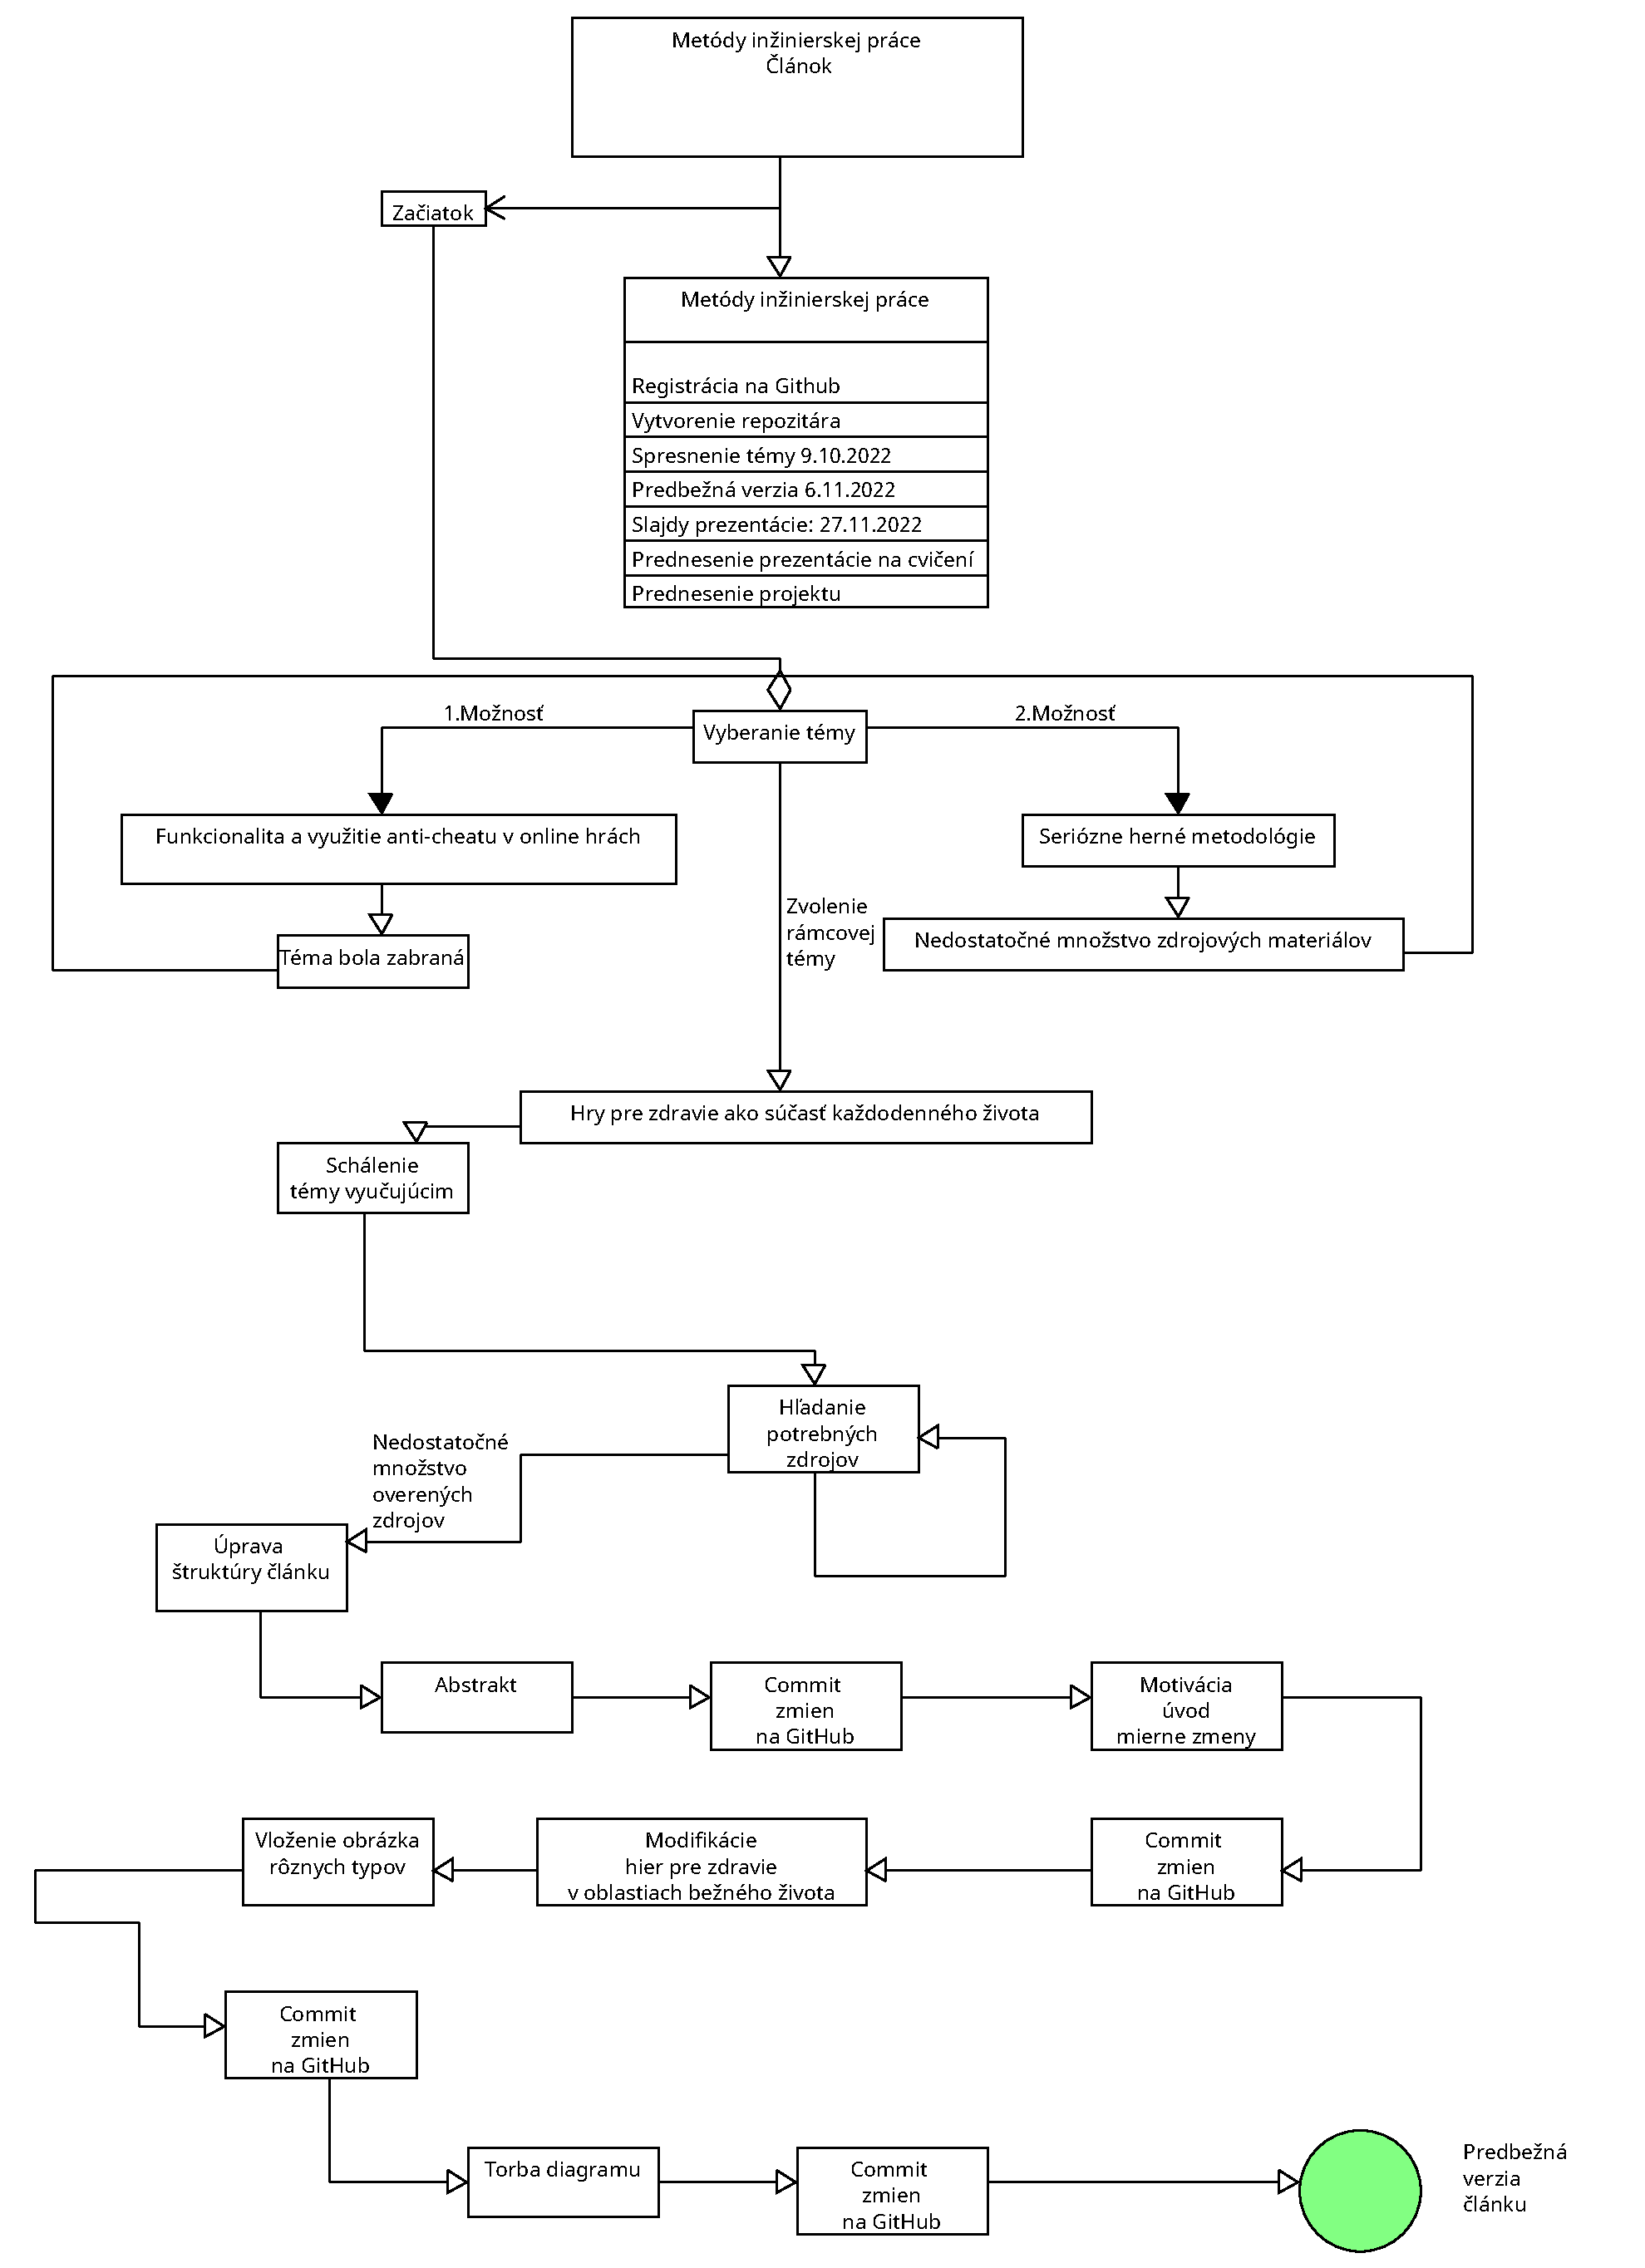
\includepdf[pages={1}]{Diagram_MIP.pdf}
\section{Proces zmien zapríčinený hrami pre zdravie}
Deti a dospievajúci sa častokrát učia počas hrania hier pomocou vizuálnej pozornosti.Vývojári do hier implikujú interaktivitu a príbeh postavy , pomocou ktorých zapríčiňujú lepšiu dejovú líniu a výsledky reflektované na zdraví ich používateľov. Mnohé štúdie preukázali , že využívanie hier stanovujúcich a plánovanie osobných cieľov nemali žiaden vplyv na spárvanie alebo klinické výsledky.Štúdia preukázala rovnaký dopad na DevOps. Vývoj hry s využitím princípov \cite{Coplien:MPD}participatívneho dizajnu viedol k nižšej účinnosti na zmeny správania a sebarozvoj ako zapojenie používateľov ako testerov bez ich začlenenia do dizajnu. Vplyv na výsledky si môže vyžadovať kombináciu rôznych techník , ktoré môžu byť ako finančne tak i časovo náročné. Hoci sa hry preukazujú ako sľubná metóda napomáhajúca ku psychickým i fyzickým zmenám , napriek tomu sú potrebné ďaľšie rozsiahle výskumy a sofistikovanejšie dizajny hier , aby boli schopné identifikovať angažovanosť, učenie a zmeny správania. 
\subsection{Dôsledky pre vývoj dieťaťa}
Bolo preukázané , že zábavné hry rozvíjajú kognitívne , behaviorálne a sociálne zručnosti ľudí už od útleho veku v rôznych vývojových obdobiach. \cite{7067095}V rámci subjektovej štúdie s deťmi od 6 do 10 rokov bolo pozorované akútne zlepšenie výkonných funkcií po hraní exergames v porovnaní so sedavou videoaktivitou. Hranie exergames na Nintende Wii zlepšilo exekutívne funkcie u adolescentov s nadváhou alebo obezitou. Pri deťoch s poruchou pozornosti a hyperaktivitou , špeciálna videohra zlepšila výkon , pamäť a vizálnopriestorovú krátkodobú pamäť. Exergaming znížil opakované zlé správanie a zlepšil kognitívnu kontrolu u detí s poruchami autistického spektra. U schizofrenikov nastalo zlepšenie neuro a sociálneho poznania . Videohry a konkrétne vážne hry môžu pozitívne ovplyvniť vývojové , najmä kognitívne výsledky u zdravých detí a u detí s rôznymi ochoreniami a postihnutiami. Kategória vážnych videohier je určená pre deti a dospievajúcich. Sú navrhnuté tak ,aby oslovili široké vekové rozpätie. Niektoré hry sú účinnejšie v niektorých vekových skupinách , ale nie v iných. Vývojovo vhodné hry zahŕňajú vhodnosť učebných osnov , včasnú a informatívnu spätnú väzbu a rovnováhu medzi zručnosťami hráčov a výzvami hry.
\subsubsection{Zainteresovaní používatelia hier pre zdravie}
Používatelia hier pre zdravie tvoria rôznorodú skupinu a možno ich rozdeliť na tých , ktorí ich majú záujem využívať na presadzovanie svojich cieľov, môžu mať propech z ich hrania alebo ich vytvárajú za účelom vykonávania výskumu v danej oblasti. Prospech z hrania videohier pre zdravie získavajú najmä rôznorodí pacienti a študenti a ich rodiny , ako i poskytovatelia zdravotnej starostlivosti.Mimo iných prospech získavajú i ľudia podielajúci sa na DevOps , akými sú napríklad projektoví manažéri , animátori , programátori, testeri a vydávatelia hier. Hry môžu zo značnej časti ovplyvniť želané zdravotné výsledky očakávané zainteresovanou stranou.S neustálym vývojom technológií dochádza ku vzniku rôznych modifikácií hier pre zdravie , ktoré umožňujú deťom byť vonku, čo minimalizuje sedenie vo vnútri a môžu zvýšiť dosiahnutú aktivitu. \cite{6662126} Iné zasa obsahujú GPS systémy na určovanie polohy , ktoré uľahčujú prvky exergamingu založené na polohe. Ku populárnym typom hier zahŕňajúcich pohyb patrí taktiež jednoznačne geocaching , ktorý je stavaný na hľadaní rôznych nálezov v prírode a ich zdieľanie v prostredí komunity. Hoci teda existuje dostatok dôkazov o tom , že hry vedú k pozitívnym výsledkom , sú potrebný ďalšie výskumy na lepšie pochopenie mechanizmov účinku a kontextových faktorov ovplyvňujúcich výsledky.
%\begin{figure*}[tbh]
\section{Záver a zhrnutie} \label{dolezita}
%\centering
%\includegraphics[scale=1.0]{diagram.pdf}
%Aj text môže byť prezentovaný ako obrázok. Stane sa z neho označný plávajúci objekt. Po vytvorení diagramu zrušte znak \texttt{\%} pred príkazom \verb|\includegraphics| označte tento riadok ako komentár (tiež pomocou znaku \texttt{\%}).

%\label{f:rozhod}
%\end{figure*}
Základným problémom , ktorý sa stáva čoraz viac popularizovaný je , hoci existuje dosatatok dôkazov o tom , že hry pre zdravie vedú k pozitívnym výsledkom ich používateľov v oblasti fyzického a psychického zdravia , ako i vo vylepšovaní kognitívnych funkcií , napriek tomu sú potrebné ďalšie výskumy pre lepšie pochopenie mechanizmov ľudského organizmu a kontextových faktorov ovplyvňujúcich zdravotné výsledky používateľov hier pre nich určených. Vo všeobecnosti sa môže zdať , že problém vlastne nejestvuje , ale bolo dokázané , že hry pre zdravie značne ovplyvňujú zdravie používateľov a umožňujú im rýchlejšiu rehabilitáciu, adaptáciu a implementáciu do bežného života. Napriek tomu i dnes na webe narazíme na rôzne pochybné názory , ktoré tvrdia presný opak ako výsledky mnohých štúdií.
\section{Reakcia na témy z prednášok}
\subsection{Spoločenské súvislosti.}
Informatika zahŕňa vývoj softvéru a hardvéru. Hardvér zahŕňa i zabudované programové vybavenie - softvér. Inžinier by mal vedieť pochopiť informáciu , interpretovať ju a aplikovať v danom kontexte , vrátane formulovania. Potrebná je technická a vedecká presnosť v písomnom a ústnom vyjadrovaní. Inžinier by mal mať schopnosť aktívne počúvať a zručne si riadiť čas, čo úzko súvisí s empatiou  a trpezlivosťou. Pri frontend developeroch sa očakáva adaptabilita i cit pre detail , vďaka ktorému dokážu vytvárať rôznorodé stránky podľa požiadaviek klienta.
\subsection{Historické súvislosti.}
\subsubsection{Polovodiče,tranzistory}
História polovodičov začína pri skúmaní elektrických vlastností materiálov na začiatoku 19. storočia - Seebeck, Faraday, Becquerell. \newline Tranzistor je trojvrstvová polovodičová súčiastka , ktorá sa skladá z troch vrstiev polovodičového materiálu. V roku 1925 navrhol Edgar Lilienfeld princíp field-effect transistor. Prvé prevedenie tranzistora bolo v roku 1947 v Bell Laboratories. Vnútorná vrstva má operačný typ nevlastnej vodivosti ako vonkajšia vrstva. Vonkajšiu vrstvu tvorí emitor a kolektor. Poznáme dva druhy tranzistorov - PNP  (dva polovodiče typu P a jeden typu N) a NPN (dva polovodiče typu N a jeden typu P). Využitie polovodičov a tranzistorov:
\begin{enumerate}
    \item{Realizácia logických obvodov(AND,OR,NOT,NAND,XOR)}
    \item{Pamäť}
    \item{Spracovanie signálu (Zosilňovač)}
\end{enumerate}
\subsection{Technológia a ľudia.}

\subsection{Git a GitHub}
Git je open source systém riadenia revízií vytvorený Linusom Torvaldsom v roku 2005 pre Linux kernel development. Využívaný je v prostredí programátorov na kolaboráciu a ukladanie zdrojového kódu počas vývoju softvéra. Dokážeme ho ovládať pomocou príkazového riadku cez GUI. Umkôžňuje nám priebežné ukladanie projektu na všetkých zariadeniach , kde bol daný repozitár naklonovaný. Na ukladanie predbežných verzií programov nám slúžia rôzny poskytovatelia hostingu na správu verzií , ako napríklad GitHub, GitLab, Bitbucket , Launchpad a rôzne íne. Základné príkazy na inicializáciu repozitára a uloženie priebežnej verzie: 
\begin{enumerate}
    \item{git init - vytvorenie repozitára}
    \item{git add . - pridanie súborov}
    \item{git commit -m "message" - poznámka pre contributorov}
    \item{git push -u origin "názov vetvy" - poslanie dát do repozitára na hosting serveri}
\end{enumerate}
\subsubsection{Čo je to GitHub?}
GitHub je hostiteľskou platformou pre Git repozitáre - remote cloud based Git repository. Podporuje kolaboráciu a  zdieľanie source kódu pri softvérovom vývoji. Podporuje správu a sledovanie histórie zmien.
\subsection{Udržateľnosť a etika.}
Udržateľnosť je v inžinierstve často zameraná na prostredie. Udržateľnosť je "riadenie,vývoj a realizácia projektovo organizovaných zmien v procesoch, zdrojoch alebo organizáciách".Udržateľnosti značne prispieva i rozvoj ,ktorý je pre spoločnosť potrebný. Spôsobuje však problémy:
\begin{enumerate}
    \item{Vyčerpávanie prírodných zdrojov - niektoré sú neobnoviteľné}
    \item{Produkcia odpadu}
    \item{Neudržateľný rozvoj}
\end{enumerate}
Stagnovať znamená nehýbať sa vo vízií podniku napred , byť na jednom mieste , nedosahovať značné úspechy.
Aby sa zdroje stíhali obnovovať je potrebné ešte pred ich vyčerpaním nájsť alternatívne zdroje , ktoré budú lepšie a obnoviteľné , ako pôvodné zdroje , príkladom sú elektrické autá.
Softvérový inžinier by mal konať tak , aby zaujal svojho klienta i zamestnávateľa. Musia pri písaní kódu udržiavať normy a integritu. Musia byť spravodliví voči svojim kolegom a podporovať ich a musia sa zúčastňovať na celoživotnom vzdelávaní týkajúcom sa výkonu ich profesie. Inžinieri vývojom softvéru objavujú lepšie spôsoby pri pomoci ostatným za pomoci technológií.
\newpage
\bibliography{literatura.bib}
\bibliographystyle{abbrv} % prípadne alpha, abbrv alebo hociktorý iný
\end{document}
